\begin{savequote}[8cm]
Far out in the uncharted backwaters of the unfashionable end of the western spiral arm of the Galaxy lies a small unregarded yellow sun. Orbiting this at a distance of roughly ninety-two million miles is an utterly insignificant little blue green planet whose ape-descended life forms are so amazingly primitive that they still think digital watches are a pretty neat idea.
  \qauthor{--- D. Adams, The Hitchhiker's Guide to the Galaxy}
\end{savequote}

\chapter{Introduction}\label{ch:1-intro}

\minitoc

How do you design and assemble something on the nanoscale? Imagine building something with lego bricks; you choose the building blocks you want and use your hands to attach them where you want them to be. However, for nanoscale objects, it is difficult to have that level of control. Instead, more success has been had by imitating nature and letting the building blocks assemble themselves.

\section{Thesis structure}
This thesis covers two related projects, both concerning the design and modular self-assembly of nanostructures. This chapter serves as an introduction to both projects, providing background on DNA and RNA self-assembly. Each project will then be introduced by a separate chapter on its relevant history and background.

The first project, introduced by Chapter \ref{ch:polycubes_intro}, covers an abstract self-assembly model called \emph{polycubes}. Chapter \ref{ch:polycubes1} details the model and presents results on the shapes that assemble when randomly sampling the input space. Chapter \ref{ch:polycubes2} presents the results on the reverse problem; given a polycube shape, what input rules will assemble it and can you minimise input complexity?

The second project takes a more detailed view of self-assembly design. Chapter \ref{ch:oxview_intro} gives a background on computer-aided design tools for nucleic acid structures, followed by an introduction of the models used to simulate such designs. Chapter \ref{ch:oxview} then presents my contributions to \emph{oxView}, a web-based tool for the visualisation, design, and integration of DNA, RNA and protein structures.


%\section{Scope of the thesis}


\section{DNA design}
Deoxyribonucleic acid (DNA) is a string-like molecule used to encode the genes of living systems \cite{calladine1997understanding}. These strings are made up of units called \emph{nucleotides}, consisting of the connecting sugar-phosphate backbone as well as one of four possible bases: \emph{adenine} (A), \emph{thymine} (T) \emph{cytosine} (C), and \emph{guanine} (G).

Through Watson-Crick base-pairing, ``A'' forms two hydrogen bonds with ``T'', while ``G'' forms three with ``C'', making DNA double-stranded. Each strand has a directionality, conventionally represented as going from the 3' to the 5' end of the strand, making the duplex anti-parallel.

The bases of the duplex are hydrophobic, while the sugar-phosphate backbone is hydrophilic, which means that the bases ``hide'' on the inside of the duplex to avoid contact with water molecules. However, the backbone distance is about 6 Å (0.6 nm), while the bases would need to be at a distance of 3.3 Å (the thickness of the base) to not leave any room for water \cite{calladine1997understanding}. To solve this, the DNA duplex forms a double helix structure with a radius of about 9 Å, placing everything at an energetically comfortable distance.

While a single double-helix is the most natural confirmation, it is possible for strands to branch into multiple junctions. For example, the Holliday junction is a junction between four double-helical arms, shown in Figure \ref{fig:holliday} in one of its possible configurations.

\begin{figure}
    \centering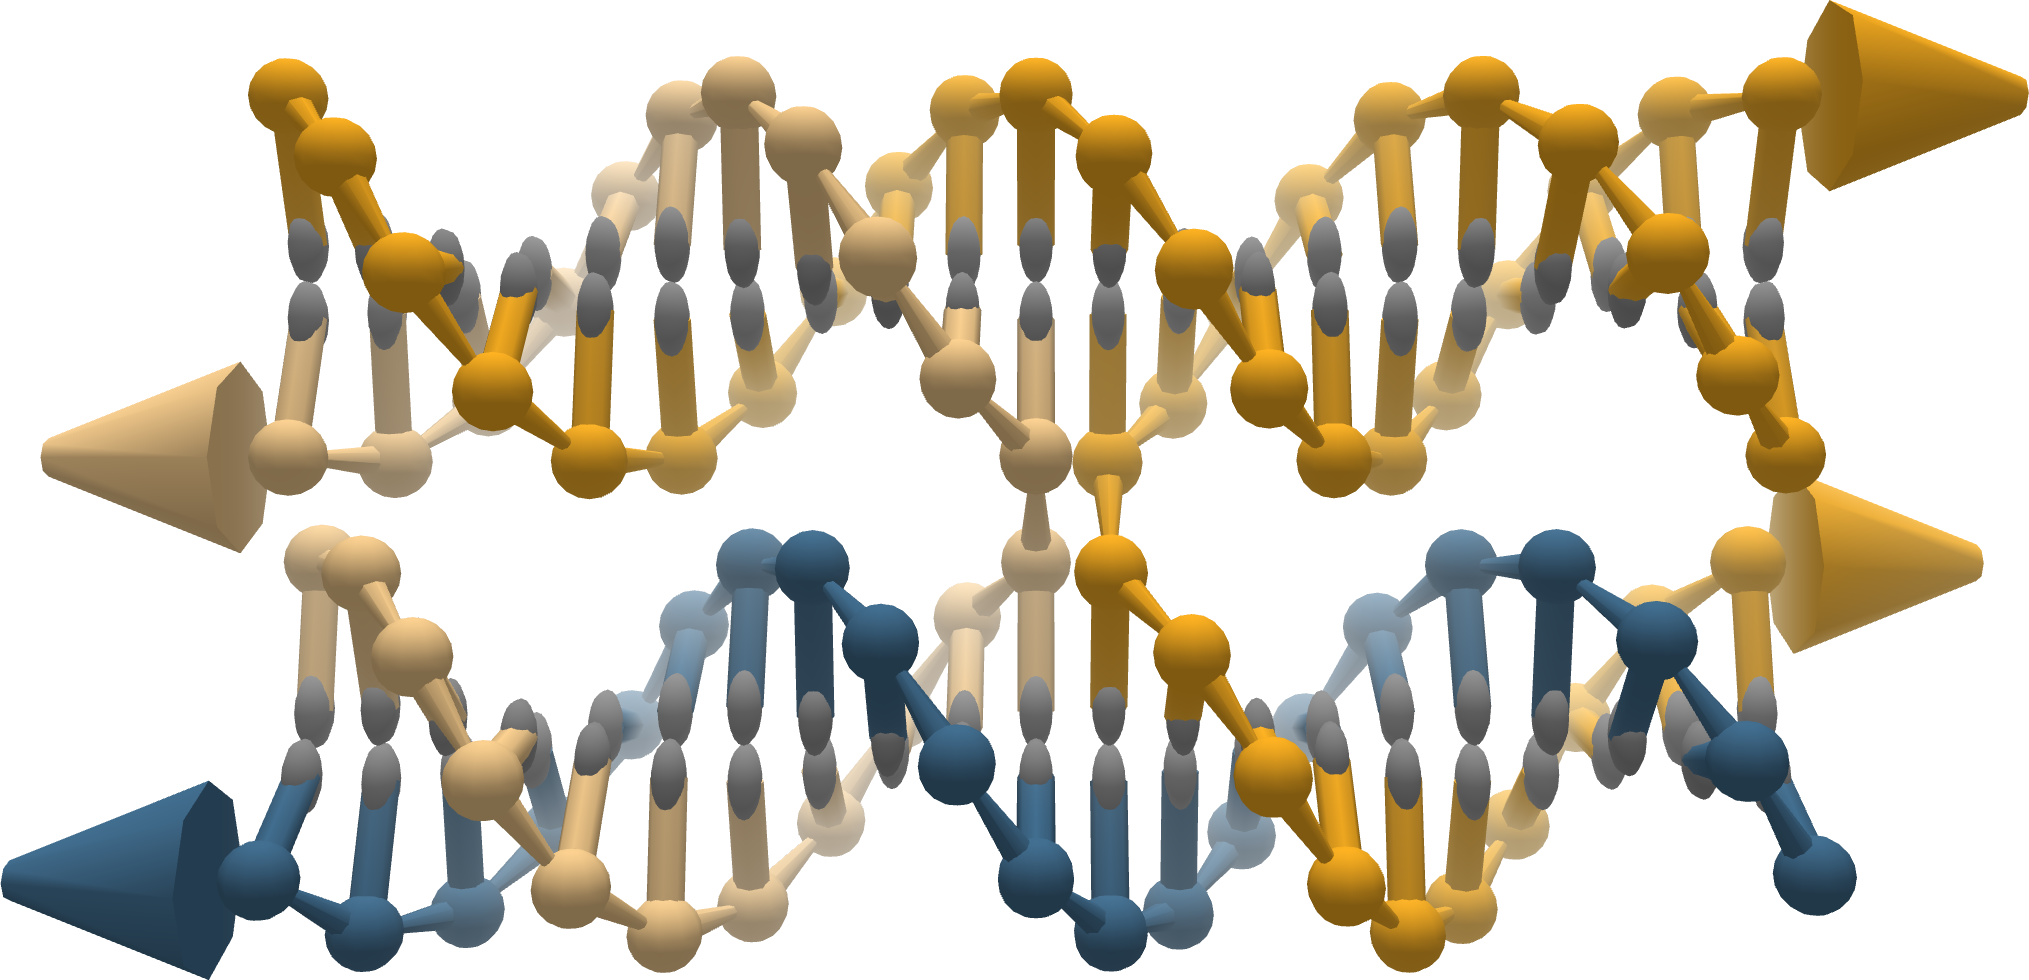
\includegraphics[width=\textwidth]{figures/holliday.png}
    \caption{Holliday junction, designed in oxView. Cones at the end indicates the 3' end of each of the four strands.}
    \label{fig:holliday}
\end{figure}

%https://www.rcsb.org/structure/1M6G

%Double-stranded DNA has a persistence length of approximately [], while single-stranded sections are much more flexible,

By designing sequences with complementary domains for the intended duplex regions, it is possible to create many different DNA motifs and structures \cite{seeman_2016}.

%% Add more here

A breakthrough in the field of structural DNA nanotechnology was the DNA origami technique \cite{rothemund2006folding} a now popular and proven method for creating larger irregular structures using DNA. The principle behind it, as illustrated in Figure \ref{fig:dnaOrigami}, is to use short staple strands to fold one long viral scaffold strand into the desired structure.

\begin{figure}
    \centering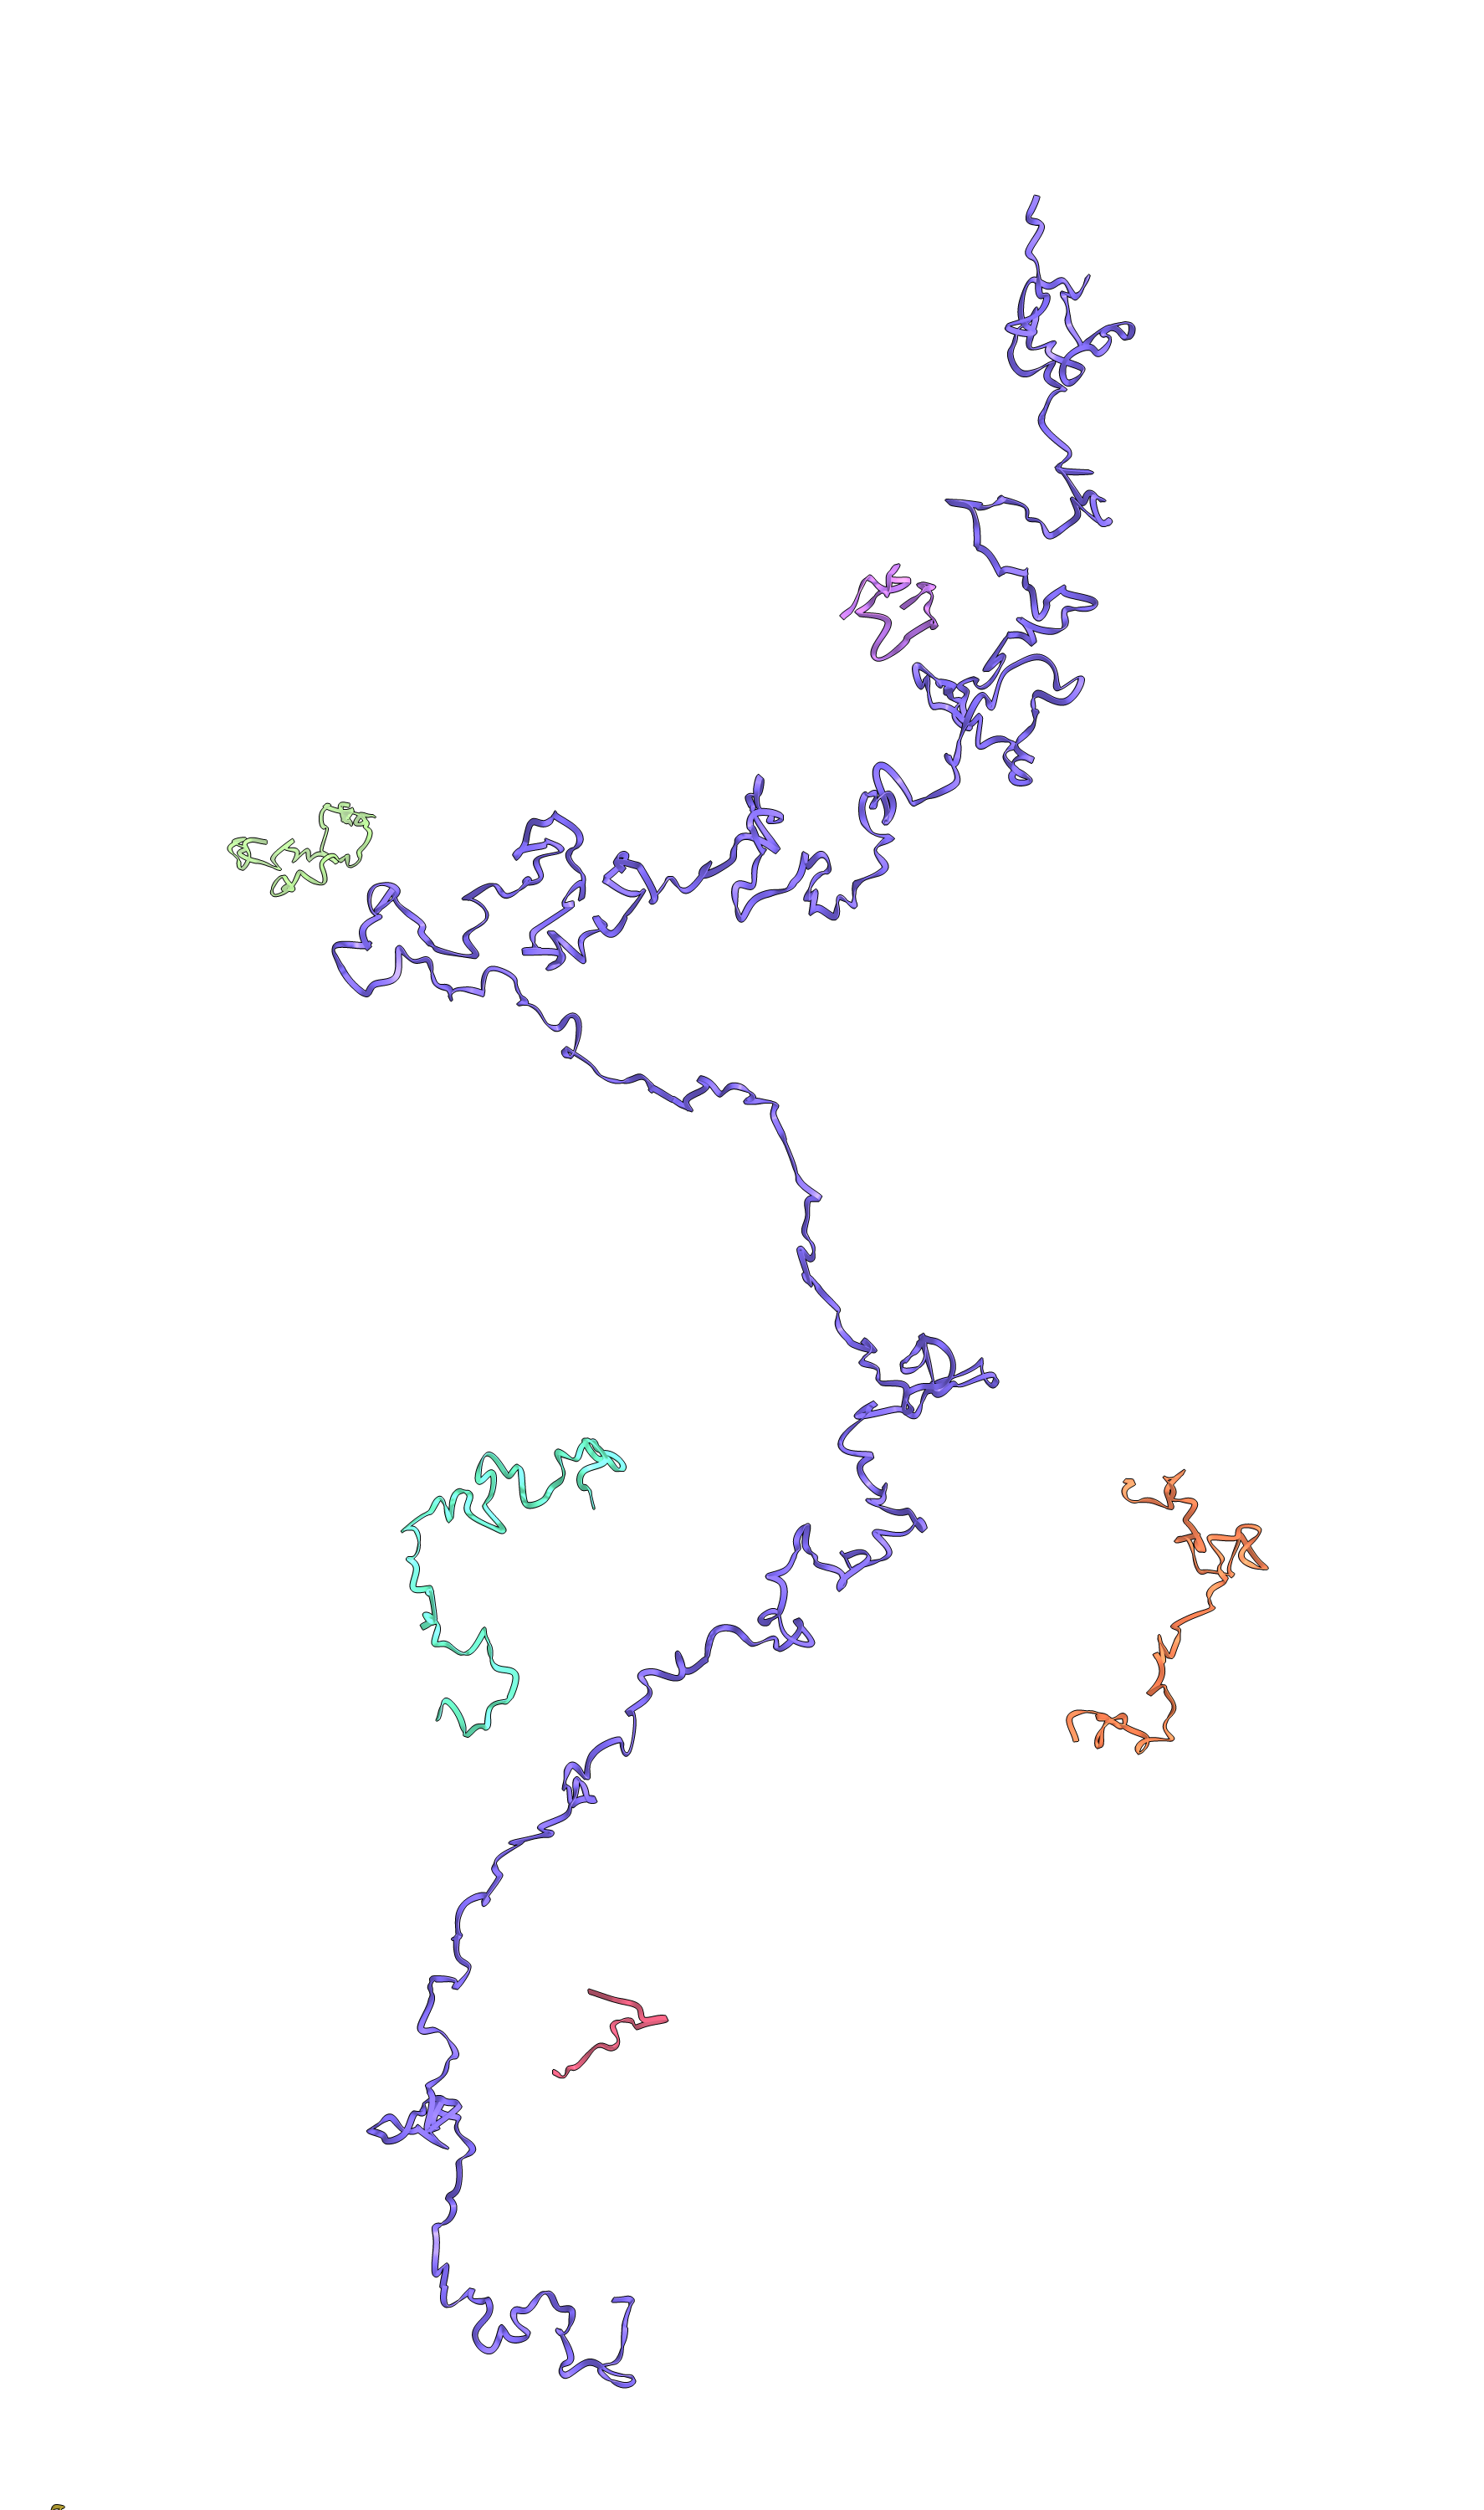
\includegraphics[width=\textwidth/5]{figures/melt/melted.png}\hfill
%    \centering\includegraphics[width=\textwidth/5]{figures/melt/intermediate2.png}\hfill
    \centering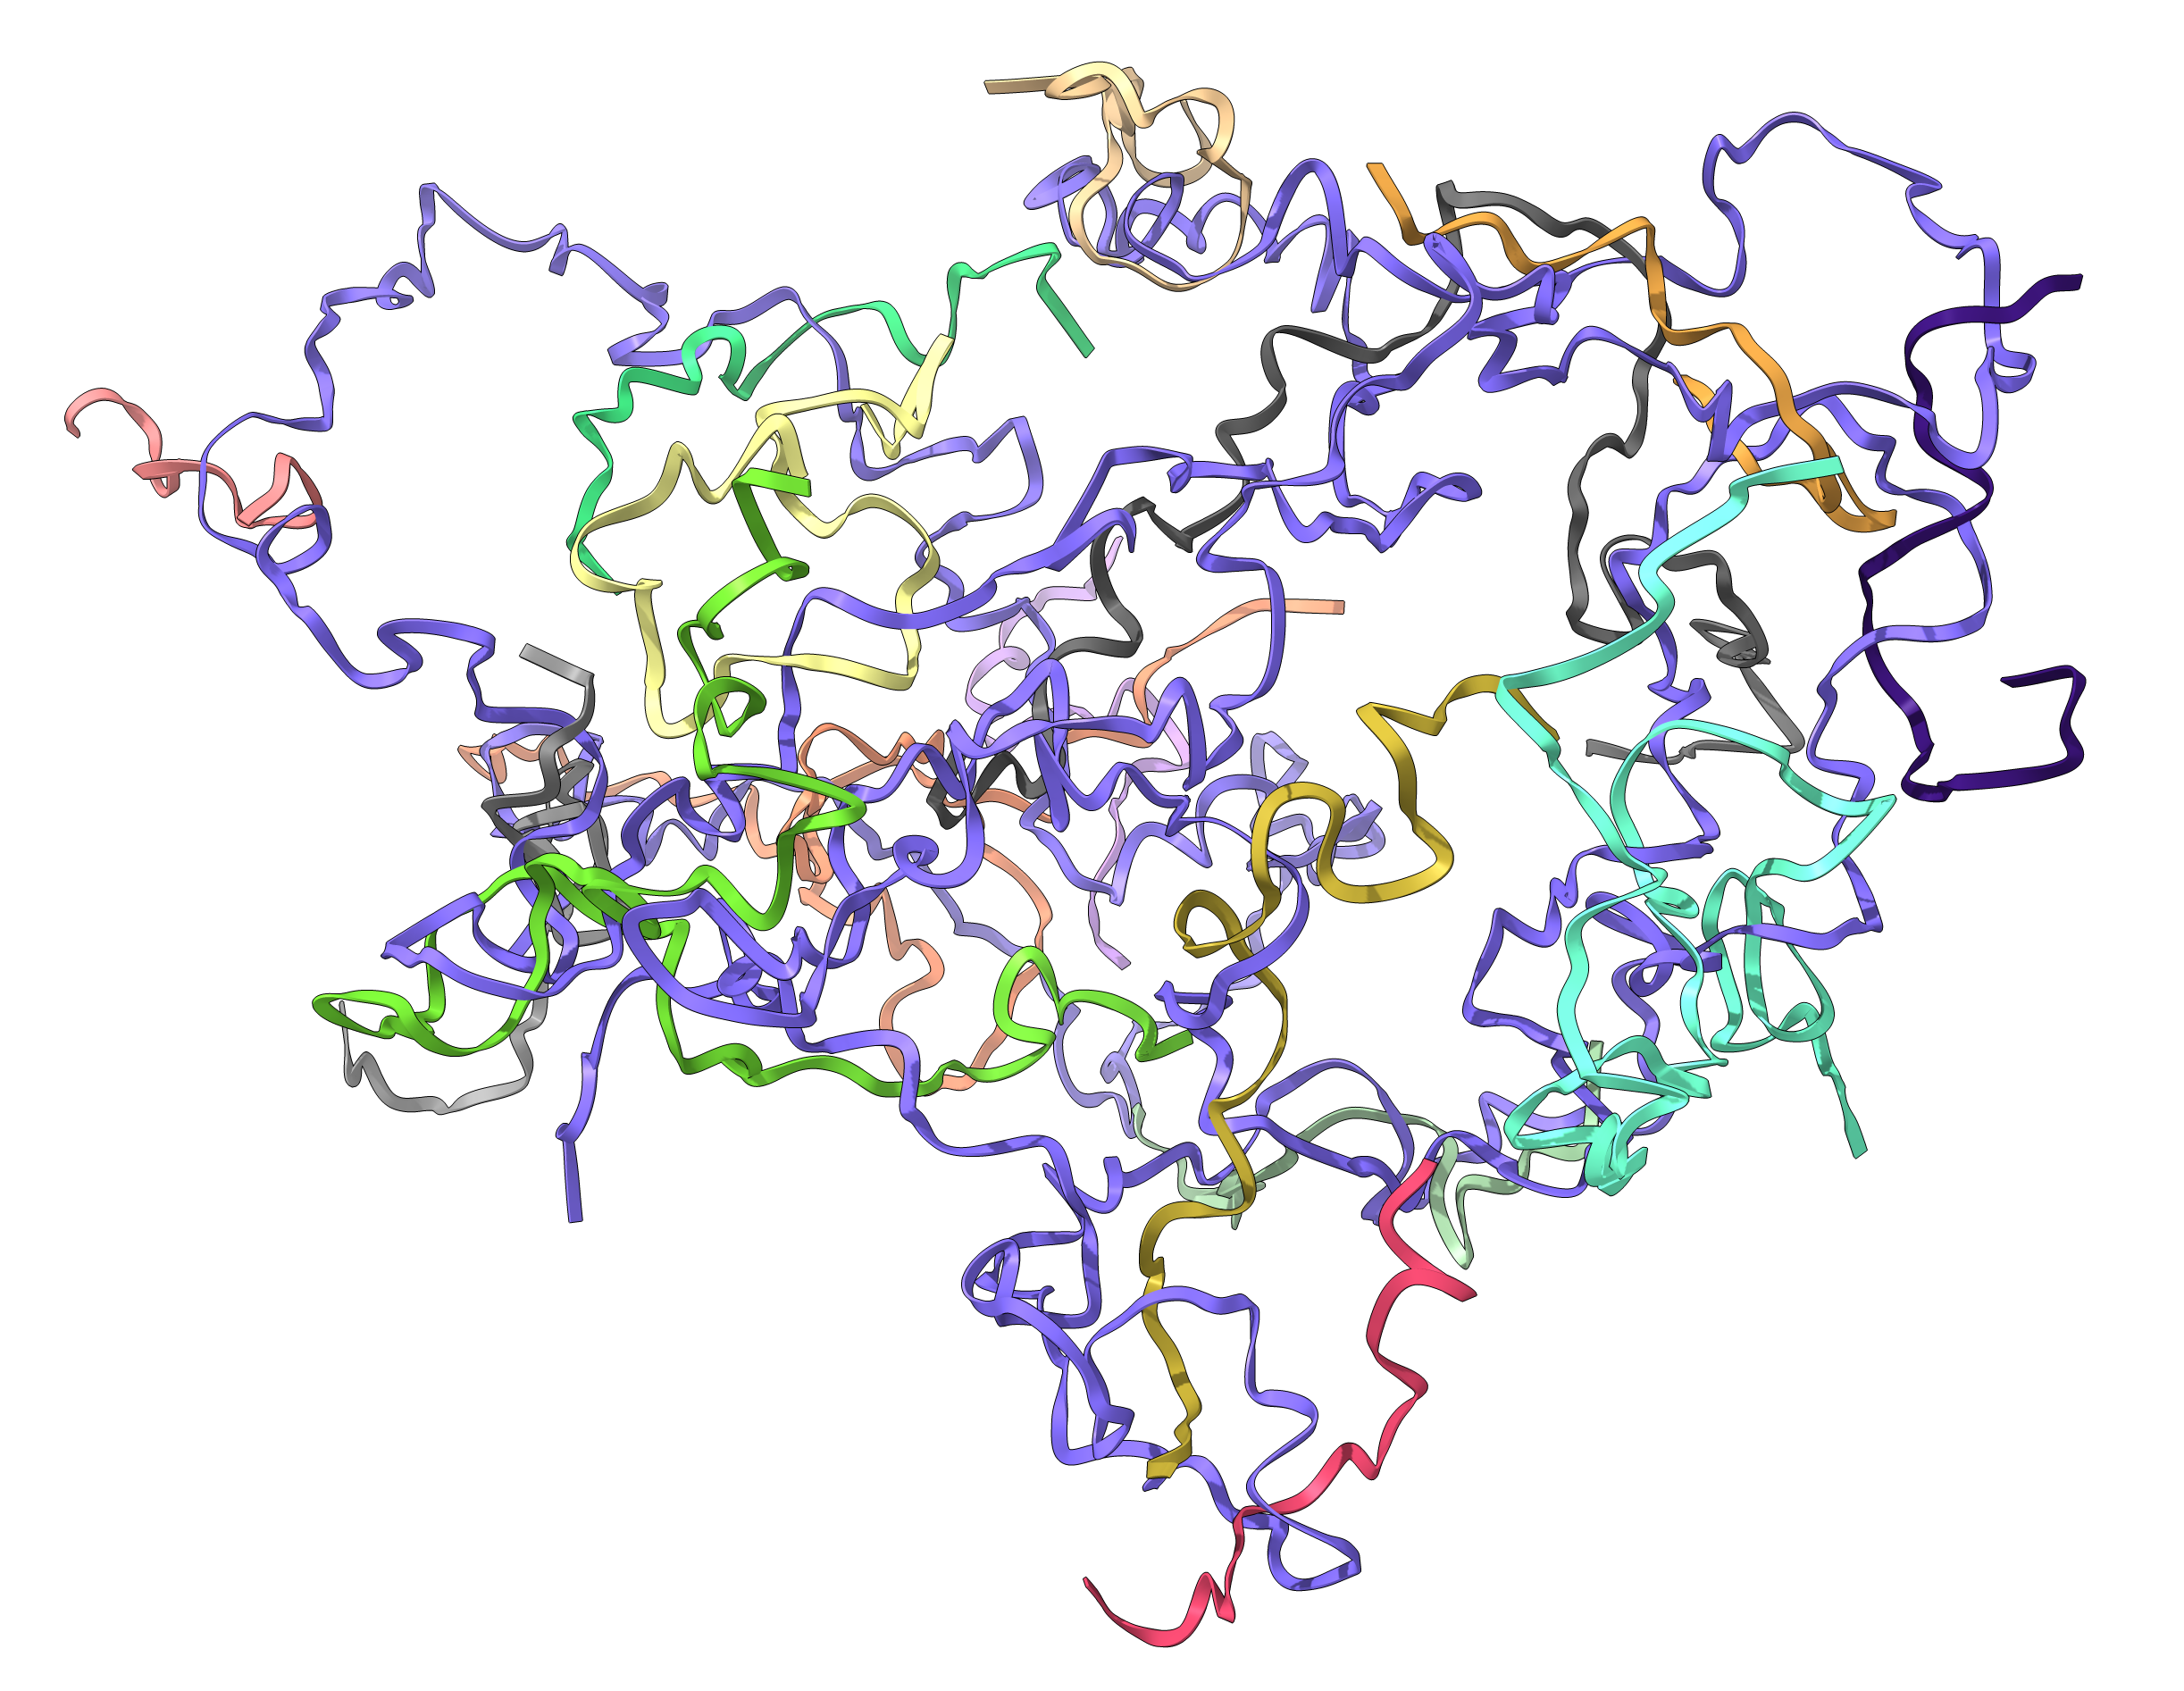
\includegraphics[width=\textwidth/3]{figures/melt/intermediate1.png}\hfill
    \centering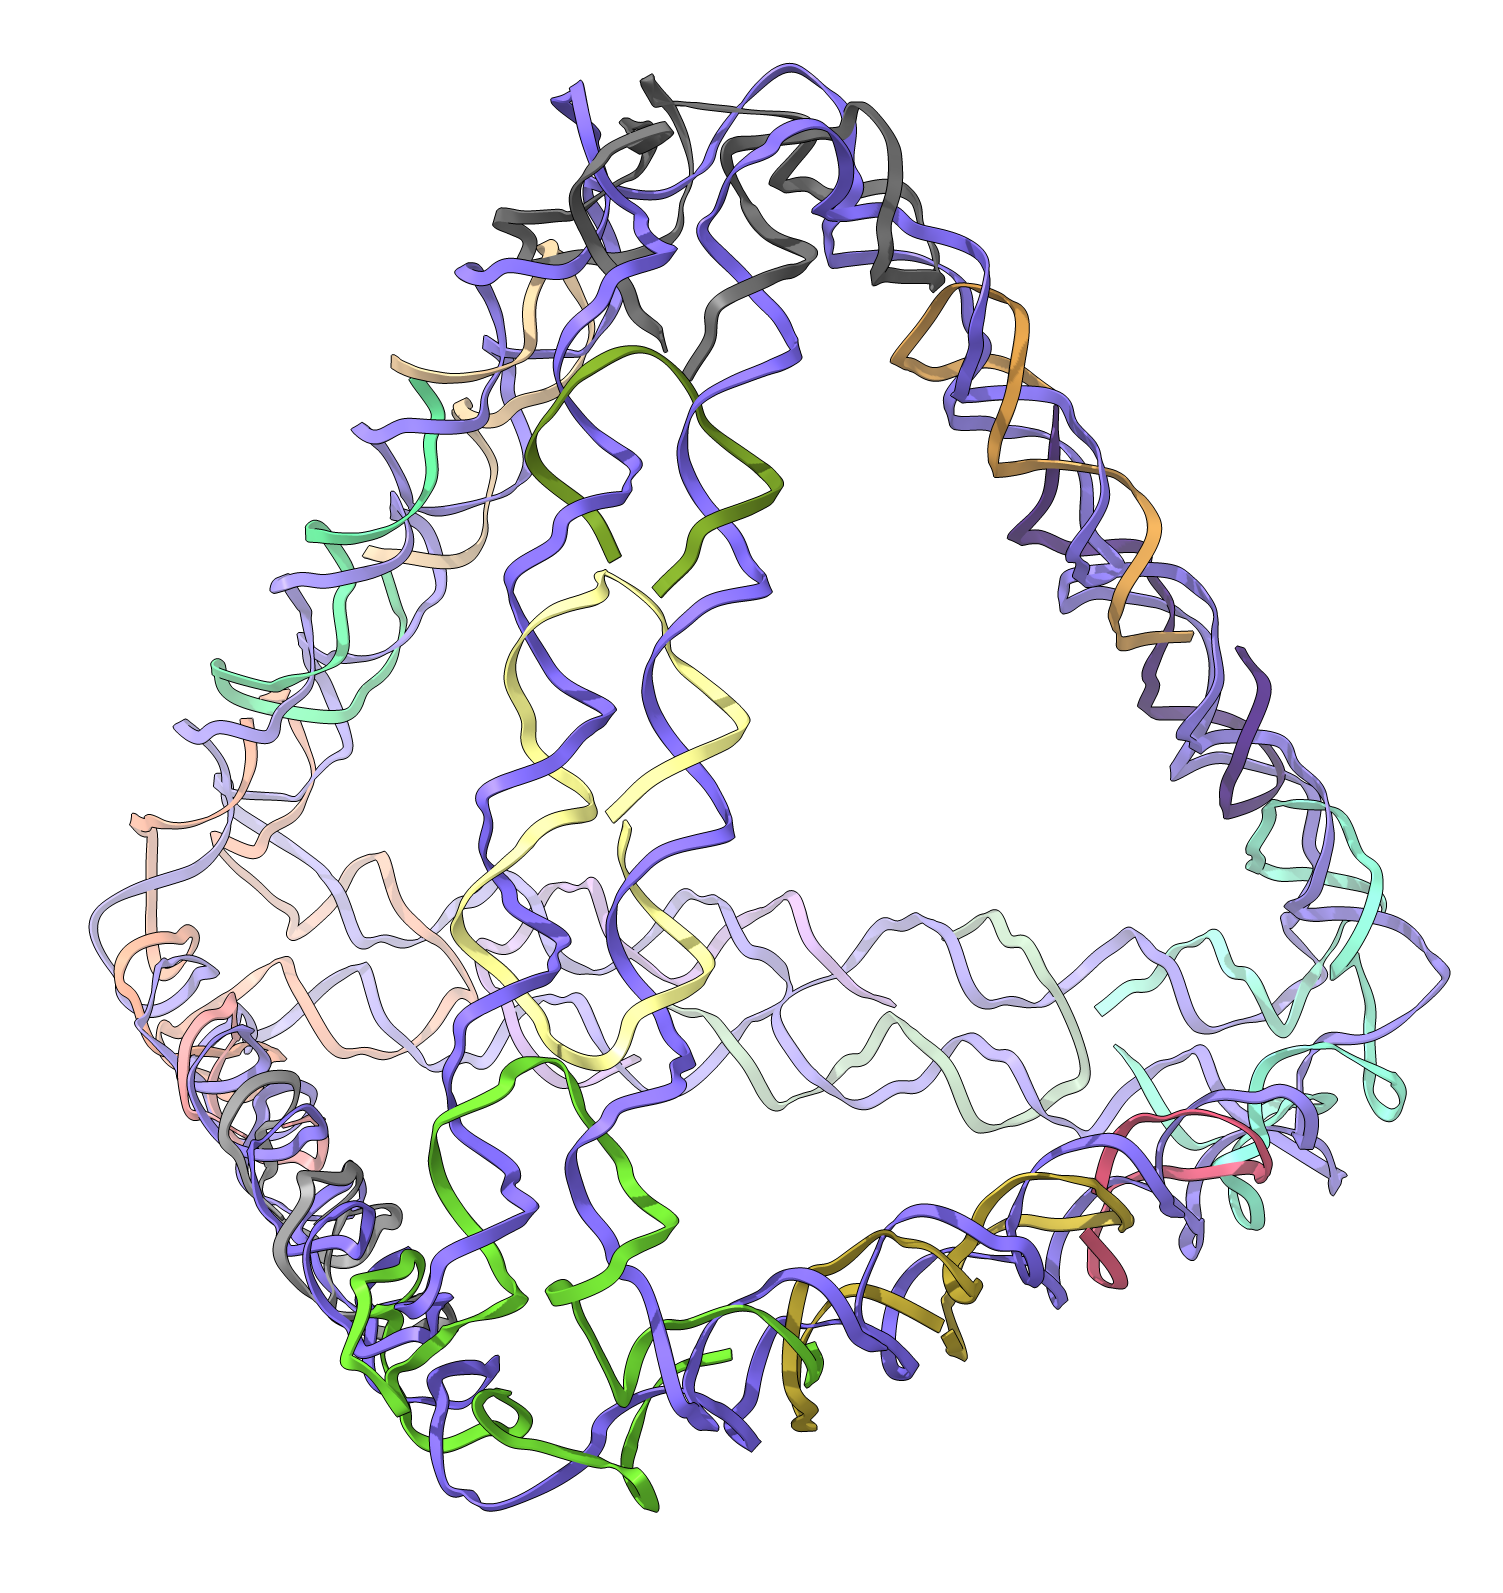
\includegraphics[width=\textwidth/3]{figures/melt/assembled.png}
    \caption{Illustration of DNA origami self-assembly of a tetrahedron. A long scaffold strand (purple), obtained from a virus, is folded into the desired shape by multiple short staple strands binding to complementary domains of the scaffold. Tetrahedron design obtained from \url{https://cando-dna-origami.org/examples/} and melted using oxDNA simulation \cite{ouldridge2010dna}.
    }
    \label{fig:dnaOrigami}
\end{figure}

Using design tools such as caDNAno\cite{cadnano}, it has become relatively easy to design structures of any given form. However, the size of the origami is limited by the length of the scaffold, which one of the motivations for researchers to investigate modular approaches, as described in Section \ref{sec:experimental_appl}.

\section{RNA design}
\label{sec:RNA_design}
Ribonucleic acid (RNA) is very similar to DNA, but with the \emph{thymine} base replaced by \emph{uracil} (U). Just like DNA, it is possible to use it as a self-assembling building material.

Biologically, DNA is transcribed into RNA by the RNA polymerase enzyme as part of gene expression. While DNA folding is easier to predict, the fact that RNA is more reactive than DNA also offers the possibility of a more useful structure; for example, by incorporating aptamers, enzymes and other such functionalities\cite{guo2010emerging}.

Geary et al., from the Andersen lab in Aarhus, demonstrated a method\cite{geary2014single, sparvath2017computer, geary2021rna} for co-transcriptionally folded RNA origami in 2014, which also enables folding \emph{in vivo}. The design used a set of tertiary RNA motifs, such as kissing hairpins and double crossovers, to fold the transcribed RNA strand into the desired structure. The Andersen lab is one of the network partners, and I have spent a two-month secondment there working with their RNA origami method.

\begin{figure}[h]
    \centering
    \begin{overpic}[width=\textwidth]{figures/rna_origami.png}
        \put(0,600){a)}
        \put(0,250){b)}
        \put(0,110){c)}
        \put(510,600){d)}
        \put(510,430){e)}
        \put(510,310){f)}
        \put(510,150){g)}
    \end{overpic}
    \caption{Co-transcriptional folding of RNA origami, adapted from \cite{geary2021rna}. a) The set of RNA motifs used as modular building blocks. b) Schematic of the modules connected to form a single strand. c) Atomistic model of the design in b). d) Shows the text-based blueprint used to create designs, while e), f), and g) shows scripts developed to aid the visualisation and preform sequence design for the origami.}
    \label{fig:rna_tiles}
\end{figure}

% "The emerging field of RNA nanotechnology121 might seem more promising in this regard because RNA is readily transcribed into a single strand in cells, which can be directly folded into a programmed nanostructure"
% https://www.nature.com/articles/nnano.2011.187

%In order achieve my goal of improving the design of modular robotic structures, simulation tools are needed to analyse the assembly of both the complete structures and of each module. During the past year, I have been working with two related sub-projects to solve both those needs, each described in the following two sections.

